\chapter{Wprowadzenie teoretyczne}

Drugi rozdział pracy poświęcony jest teoretycznemu omówieniu podstawowych pojęć związanych z równoległością i~współbieżnością, w tym w omówieniu działania wątków we współczesnych systemach operacyjnych, zdefiniowaniu typowych problemów występujących w systemach współbieżnych oraz przedstawieniu najważniejszych założeń różnych modeli współbieżności dostępnych w ramach środowiska JVM, w szczególności klasycznego modelu współbieżności oferowanego w ramach Thread API, modelu opartego o pule wątków (dostępnego w~ramach interfejsu \texttt{ExecutorService})
% , modelu opartego o podział zadań i łączenie uzyskanych wyników (Fork/Join Framework)
 oraz reaktywnego modelu współbieżności oferowanego przez Reactive Streams i RxJava.

\section{Podstawowe pojęcia}

\subsection{Współbieżność a równoległość}

Jak podają Tanenbaum i Bos \cite{tanenbaum2023}, \emph{współbieżność} (ang. \emph{concurrency}) oznacza zdolność systemu do obsługi wielu zadań w taki sposób, że ich wykonywanie nakłada się w czasie, nawet jeśli w danym momencie wykonywane jest tylko jedno z nich. \emph{Równoległość} (ang. \emph{parallelism}) oznacza obsługę wielu zadań w tym samym czasie przy wykorzystaniu wielu jednostek obliczeniowych.

Innymi słowy, współbieżność odnosi się do strukturalnej organizacji systemu oraz sposobu modelowania i zarządzania wieloma zadaniami, natomiast równoległość oznacza ich faktyczne, jednoczesne wykonywanie na wielu procesorach lub rdzeniach. We współczesnych systemach operacyjnych zadania te są wykonywane w ramach \emph{procesów} i \emph{wątków}.

% dodać coś jeszcze?

\subsection{Pojęcie i zasada działania wątków}

We współczesnych systemach operacyjnych najważniejszą abstrakcją umożliwiającą współbieżne wykonywanie operacji są \emph{procesy} (ang. \emph{processes}). Jak wskazują Tanenbaum i Bos \cite{tanenbaum2023}, procesy umożliwiają przekształcenie jednej jednostki obliczeniowej (CPU) na wiele wirtualnych jednostek, w ramach których mogą współbieżnie wykonywać zadania poprzez umiejętność CPU do szybkiego przełączania się między procesami.

W celu umożliwienia bardziej efektywnej współbieżności wewnątrz pojedynczego procesu, współczesne systemy operacyjne oferują \emph{wątki} (ang. \emph{threads}), definiowane jako lżejsze jednostki wykonania. Wątki działają w obrębie jednego procesu i~współdzielą z nim przestrzeń adresową oraz zasoby, zachowując jednocześnie własny kontekst wykonania \cite{tanenbaum2023}. Różnice między procesem a wątkiem prezentuje rysunek \ref{fig:process-thread-diff}.

\begin{figure}[ht]
    \centering
    \begin{subfigure}[b]{0.49\textwidth}
        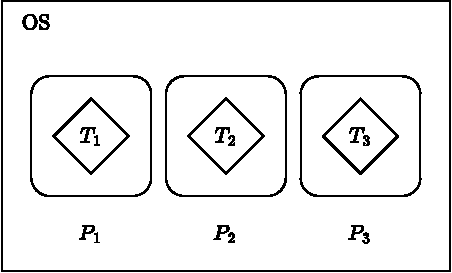
\includegraphics[width=\textwidth]{rozdzialy/rozdzial2/img/processes.pdf}
        \caption{trzy jednowątkowe procesy}
        \label{fig:process-thread-diff:processes}
    \end{subfigure}
    \hfill
    \begin{subfigure}[b]{0.49\textwidth}
        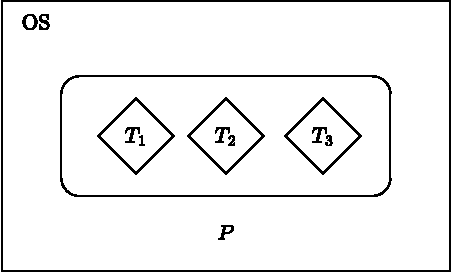
\includegraphics[width=\textwidth]{rozdzialy/rozdzial2/img/threads.pdf}
        \caption{jeden trzywątkowy proces}
        \label{fig:process-thread-diff:threads}
    \end{subfigure}
    \caption{Rozróżnienie procesów i wątków w systemie operacyjnym}
    \source{opracowanie własne na podstawie \cite{tanenbaum2023}}
    \label{fig:process-thread-diff}
\end{figure}

\noindent
Mimo że oba systemy przedstawione powyżej operują na trzech wątkach $T_1$, $T_2$ i~$T_3$, wątki na rysunku \ref{fig:process-thread-diff:processes} operują na odrębnych przestrzeniach adresowych, podczas gdy wątki przedstawione na rysunku \ref{fig:process-thread-diff:threads} działają w obrębie jednej (wspólnej) przestrzeni adresowej, co wynika z faktu operowania wewnątrz jednego (wspólnego) procesu $P$.

% dodac krotki akapit o zasadzie dzialania watkow

\section{Problemy występujące w systemach współbieżnych}
\label{sec:concurrency-problems}
% spisac i opisac najwazniejsze problemy: deadlock, starvation, synchronizacja, sekcja krytyczna, ... (poszukac innych/lepszych)

% race condition, sekcja krytyczna, deadlock, starvation, synchronizacja
% Przeczytac z Goetza poniższe rozdziały: 1.3, cały 2, 5.1, podsumowanie części I (s. 128), 6, 7, 8, 10, 

% mutual exclusion (Ben Ari, 2.2)
% race condition, pamięć współdzielona (rozwiązanie: synchronizacja) (1.3 + 2.2.1)
% problemy żywotności: deadlock (10.1), livelock (10.3.3), starvation (10.3.1) - opisać pojęcie żywotności (1.3.2)
% problemy związane z wydajnością (performance hazards) (1.3.3 + 11)

Mimo wielu zalet wykorzystania wątków do współbieżnego wykonywania zadań, podejście to wiąże się z istnieniem wielu problemów obecnych w systemach współbieżnych. Wiele publikacji wskazuje na cztery główne kategorie problemów: problemy związane z mechanizmem wzajemnego wykluczania i synchronizacją wątków, \emph{race condition} i~pamięć współdzieloną, problemy żywotności, takie jak \emph{deadlock}, \emph{livelock} i \emph{starvation}, a także problemy związane z wydajnością. Poniżej opisano charakterystykę każdego z nich.

\subsection{Wzajemne wykluczanie i synchronizacja}
Ben-Ari \cite{benari1982} definiuje wzajemne wykluczanie (ang. \emph{mutual exclusion}) jako jeden z~najważniejszych problemów programowania współbieżnego z racji bycia abstrakcją dla wielu problemów związanych z synchronizacją wątków.

Herlihy i Shavit \cite{herlihy2012} wskazują, że wątki \emph{wykluczają się wzajemnie}, jeśli co najmniej dwa z nich próbują równocześnie wykonać wspólny blok kodu, nazywany \emph{sekcją krytyczną} (ang. \emph{critical section}), ale w danym momencie tylko jeden z nich ma dostęp do sekcji krytycznej.

% dodać coś jeszcze

\subsection{\emph{Race condition} i pamięć współdzielona}

\subsection{Problemy żywotności: \emph{deadlock}, \emph{livelock}, \emph{starvation}}

Goetz \cite{goetz2006} definiuje \emph{żywotność} (ang. \emph{liveness}) jako właściwość systemu, która zapewnia, że koniec końców pewna własność się wydarzy, czyli że system nie będzie pozostawał w stanie zawieszenia lub bezczynności. Problemy żywotności występują, gdy system nie jest w stanie kontynuować wykonywania zadań z powodu wzajemnych zależności między wątkami lub braku zasobów. Najpopularniejszymi z nich są \emph{deadlock}, \emph{livelock} i \emph{starvation}.

\subsection{Problemy związane z wydajnością}

\section{Modele współbieżności w środowisku JVM}

Środowisko JVM oferuje wiele różnych modeli umożliwiających tworzenie współbieżnych aplikacji. Ta część poświęcona jest omówieniu najpopularniejszych podejść, w tym podstawowego (i chronologicznie pierwszego) modelu, dostępnego w~ramach Thread API, modelu opartego o wykorzystanie wzorca projektowego \emph{Pula} (ang.~\emph{Pool}), dostępnego w ramach interfejsu \texttt{ExecutorService},
% modelu opartego o~framework Fork/Join, realizującego podział zadań i łączenie wyników,
 a~także modelu reaktywnego.

\subsection{Klasyczny model współbieżności (Thread API)}
\label{sec:thread-api}
% okreslenie tego rodzaju watkow jako platform thread, opisac ze watki platformowe w JVM mapuja sie 1:1 na watki OS, opisac wady tego podejscia (tworzenie watku jest kosztowne czasowo i pamieciowo)

\subsection{Model oparty o pule wątków (\texttt{ExecutorService})}
% Goetz 8.2 - rozmiar puli wątków 

% \subsection{Model oparty o podział zadań i łączenie wyników (Fork/Join Framework)}

\subsection{Reaktywny model współbieżności (Reactive Streams, Project Reactor, RxJava)}
\label{sec:reactive}
